\subsection{Rebrickable}
  Rebrickable \autocite{rebrickable:homepage} je webová aplikace sloužící ke správě sbírek LEGO součástek a stavebnic. Umožňuje uživateli prohlížení rozsáhlé databáze obsahující více než 11 500 oficiálních stavebnic a více než 25 000 unikátních součástek prodávaných společností LEGO od roku 1950 po současnost \autocite{rebrickable:about}. 

  \subsubsection{Poskytovaná data}  
  Rebrickable svou databázi zpřístupňuje dvěma způsoby. Jedním způsobem je pravidelný (měsíční) výpis z~databáze formou tabulek ve formátu \textit{\gls{CSV}}. Druhou možností je získávání dat přes veřejné \gls{API}. Struktura tabulek \textit{\gls{CSV}}, které jsou ke stažení ze stránek \autocite{rebrickable:download} je znázorněna na obrázku \ref{diagram-rebrickable}.

  \subsubsection{Číslování součástek}
  Velkou výhodou použití dat služby Rebrickable je systém číslování součástek, který vychází z~číslování u~knihovny \textbf{LDraw} \autocite{rebrickable:faq}. To ušetří velké množství práce při mapování součástek z~databáze Rebrickable na součástky knihovny \textbf{LDraw}. 
  
  \subsubsection{Licence}
  Data aplikace jsou veřejně dostupná pro jakékoliv účely, včetně komerčních. Autoři aplikace pouze žádají o~zveřejnění prohlášení o~původu dat. \autocite{rebrickable:terms}
  
  \begin{figure}[htbp]
    \centering
    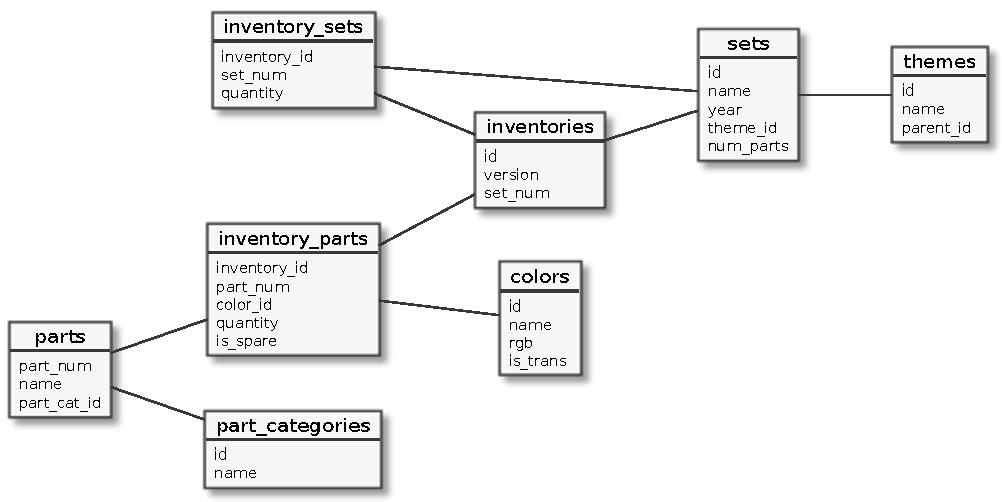
\includegraphics[width=\textwidth,height=\textheight,keepaspectratio]{pdfs/rebrickable_schema}
    \caption{Diagram schématu, Rebrickable \autocite{rebrickable:download}\label{diagram-rebrickable}}
  \end{figure}

  \subsubsection{Závěr}
  Pro získání dat o~inventářích jednotlivých stavebnic bude využita databáze služby Rebrickable ve formě \textit{\gls{CSV}} tabulek. Využití kompletních dat je pro účely aplikace optimálním řešením. Na rozdíl od varianty dynamického získávání dat přes \gls{API} umožňuje předem připravené namapování součástek na 3D modely a celkově rychlejší přístup k~datům.